\section{Inference Engine}
\label{sec:cpig}

We implemented a program that leverages data from \cref{table:impls1,table:non-impls}
to infer new implications and non-implications among fairness notions.
See \cref{fig:cpigjs} for the program's screenshot.

\begin{figure}[htb]
\centering
\ifx\version\versionIjcai
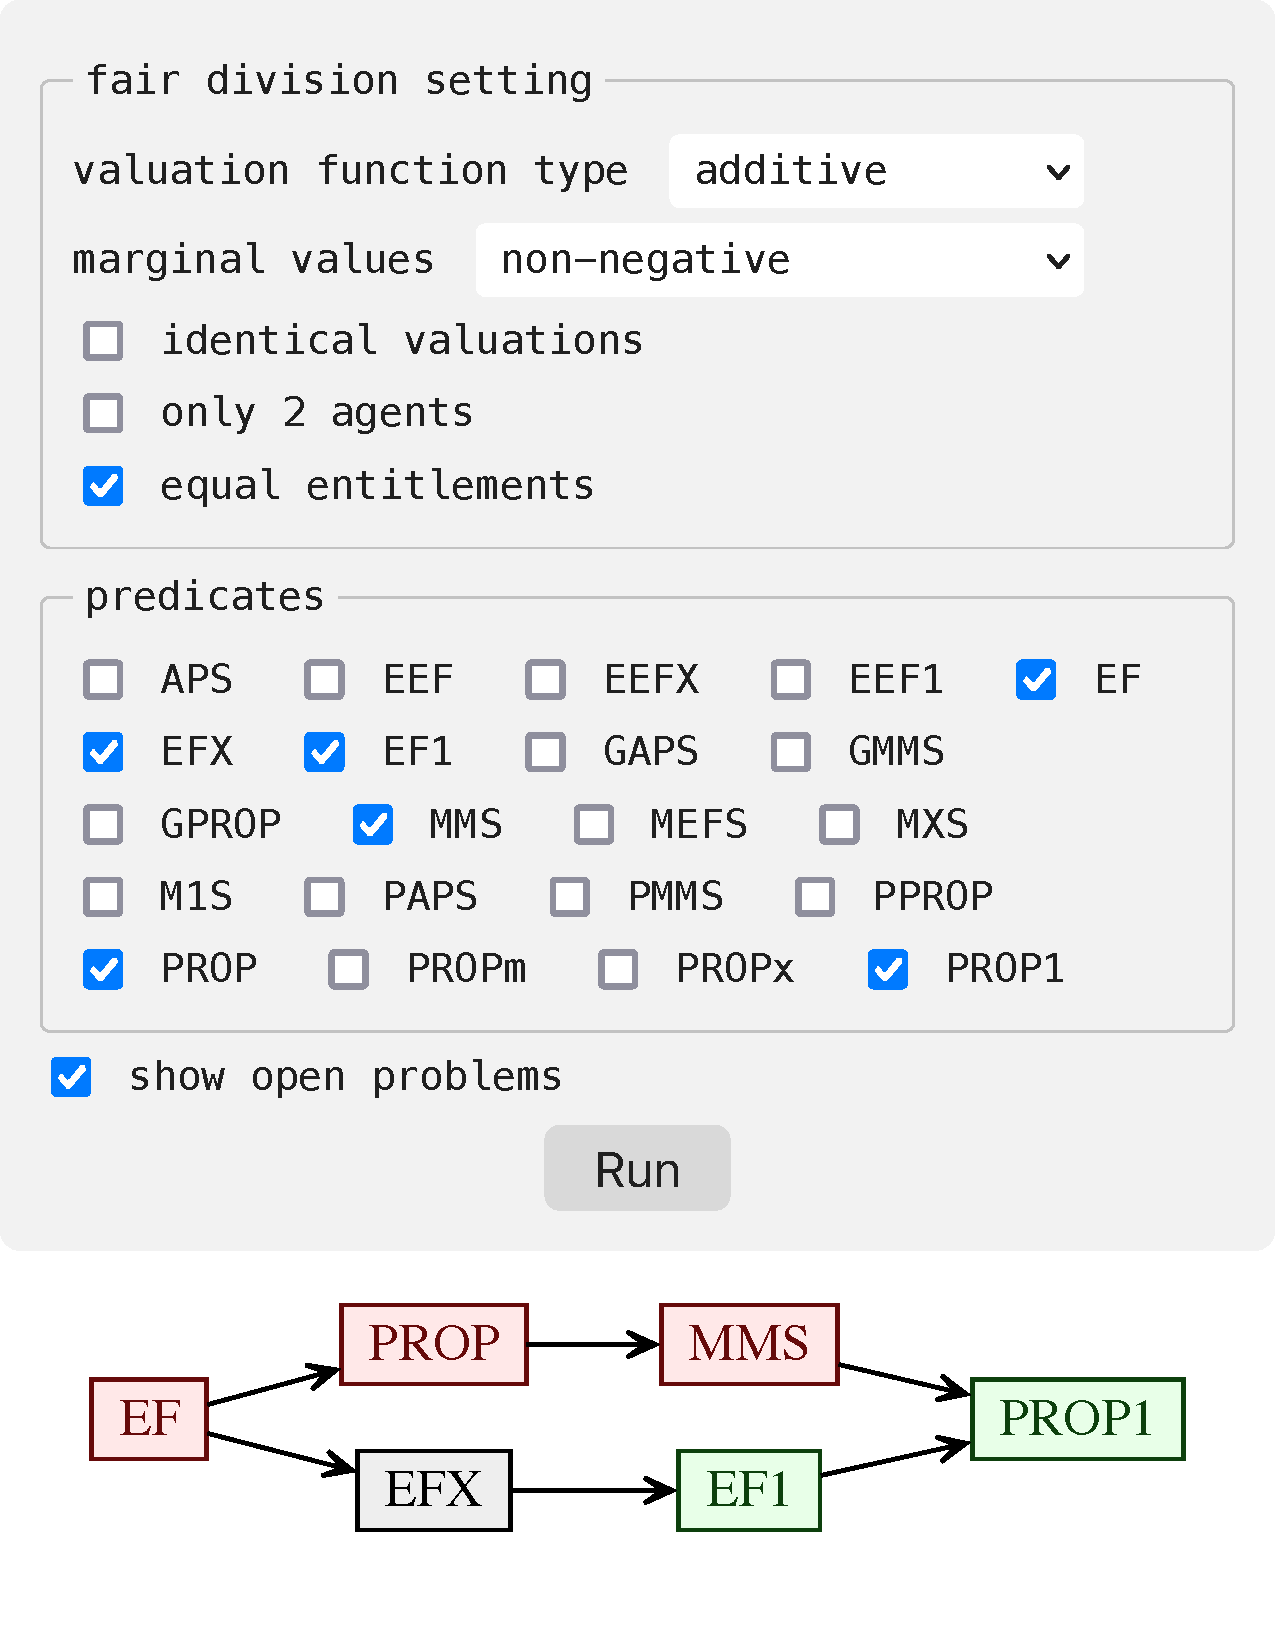
\includegraphics[width=0.8\linewidth]{figs/cpigjs-fd-ui2.pdf}
\else
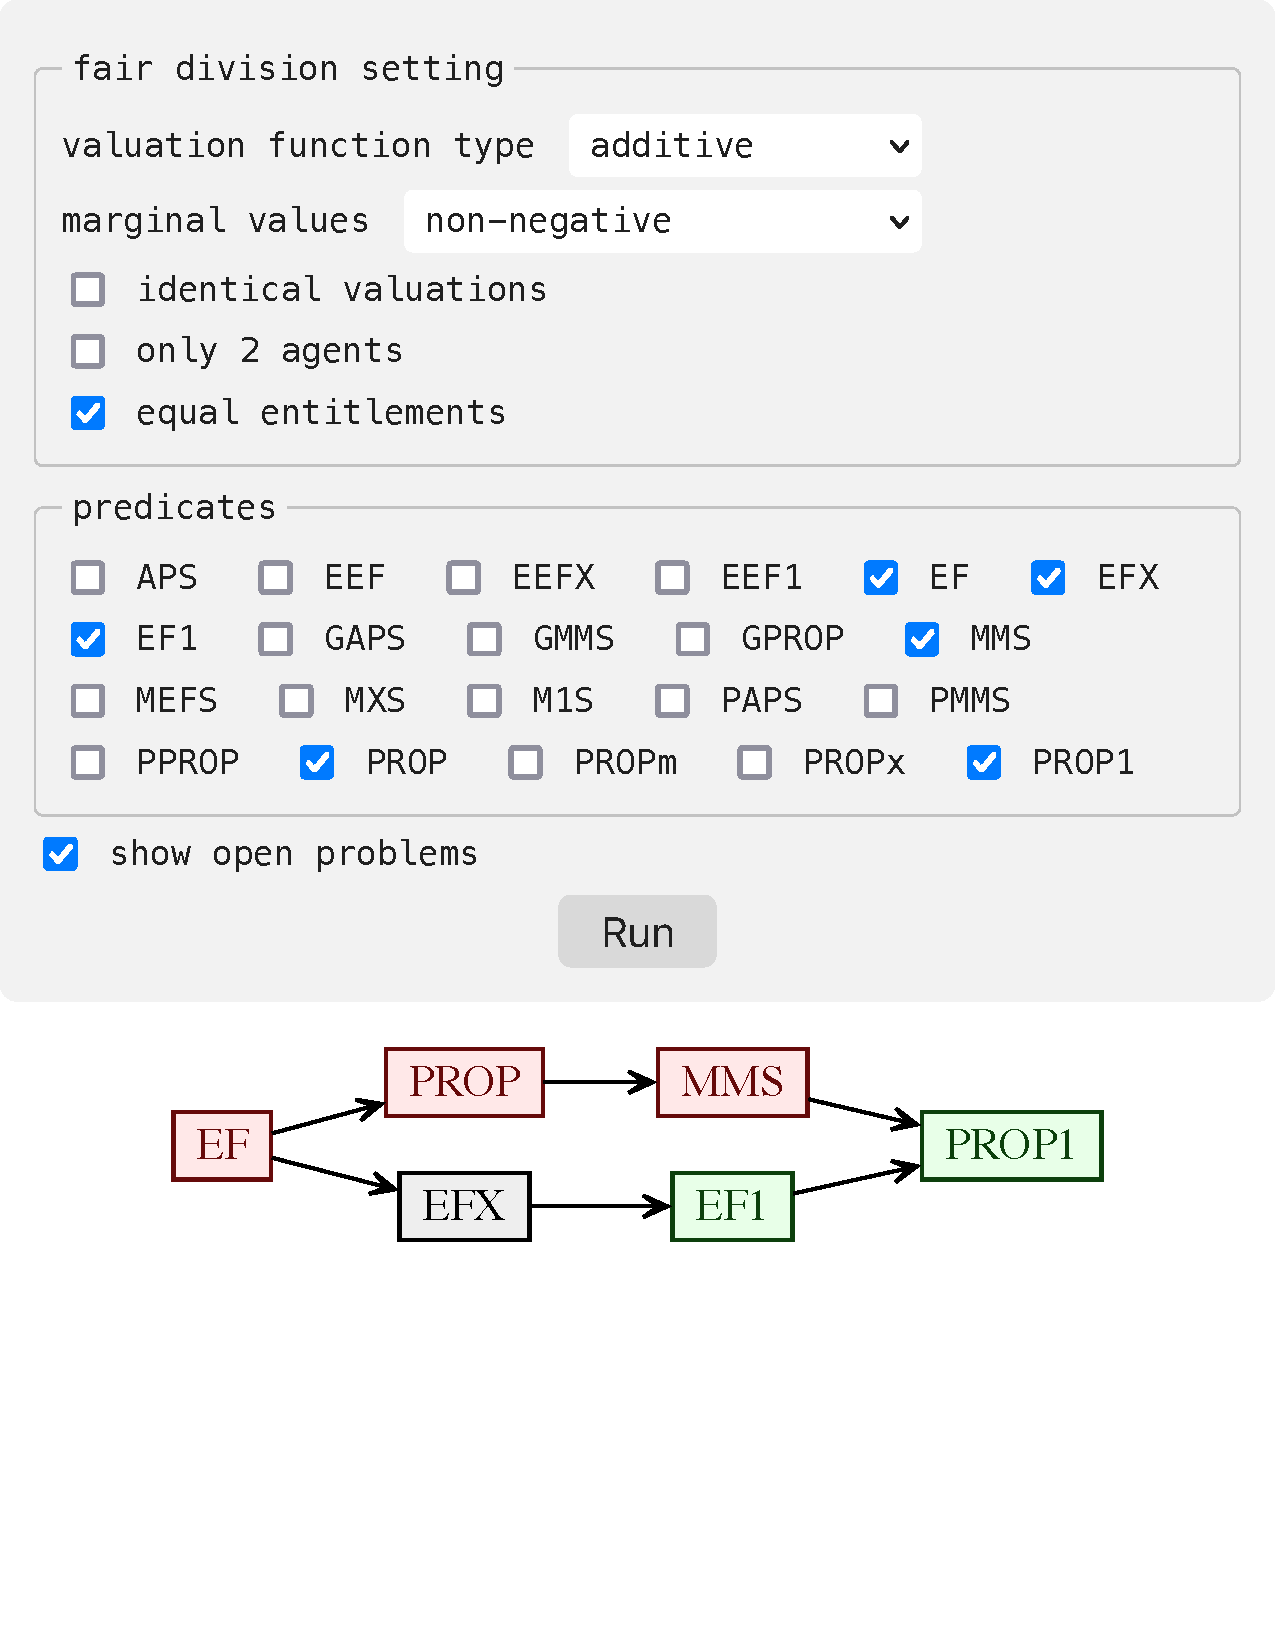
\includegraphics[width=0.6\textwidth]{figs/cpigjs-fd-ui.pdf}
\fi
\caption[Screenshot from cpigjs]{
Screenshot from the inference engine's web interface for fair division.}
\label{fig:cpigjs}
\end{figure}

Our program is not limited to just fair division.
It can be used more broadly for \emph{conditional predicate implications}.
A \emph{predicate} is a function whose co-domain is $\mathbb{B} \defeq \{\mathtt{true}, \mathtt{false}\}$.
Given two predicates $\phi_1, \phi_2: \Omega \to \mathbb{B}$,
we say that $\phi_1$ \emph{implies} $\phi_2$ conditioned on $S \subseteq \Omega$,
denoted as $\phi_1 \fimplies_S \phi_2$,
if $\phi_1(x) \fimplies \phi_2(x)$ for all $x \in S$.
In fair division, $\Omega$ is the set of all pairs $(\Ical, A)$,
where $\Ical$ is a fair division instance and $A$ is an allocation for $\Ical$.
A fair division setting is a subset of $\Omega$,
and fairness notions are predicates over $\Omega$.

The inference engine takes as input a tuple $(\Fcal, \Phi, I, C)$.
$\Fcal$ is a set family over a ground set $\Omega$.
    Since $\Omega$ can be uncountable, we represent sets in $\Fcal$ implicitly.
    Given $S_1, S_2 \in \Fcal$, we should be able to efficiently tell whether $S_1 \subseteq S_2$.
$\Phi$ is a set of predicates over $\Omega$.
$I$ is a set of \emph{conditional implications}, i.e., a set of triples
    $(\phi_1, \phi_2, S) \in \Phi \times \Phi \times \Fcal$
    where $\phi_1 \fimplies_S \phi_2$.
$C$ is a set of \emph{conditional counterexamples}, i.e., a set of triples
    $(\phi_1, \phi_2, S) \in \Phi \times \Phi \times \Fcal$,
    where $\phi_1(x) \nfimplies \phi_2(x)$ for some $x \in S$.

We repeatedly query the inference engine with a set $S \in \Fcal$,
and it outputs all possible implications and counterexamples conditioned on $S$,
even those that are not explicitly present in $I$ and $C$.
In our implementation, we represent the output as a Hasse diagram.

The inference engine works in two steps.
In step 1, we find all implications conditioned on $S$.
To do this, we simply select implications from $I$ that are conditioned on
supersets of $S$, and compute their transitive closure.
In step 2, we find all counterexamples conditioned on $S$.
To do this, for each $(\phi_1, \phi_2, T) \in C$,
we first find all implications conditioned on $T$ like in step 1.
If $\phi_1 \fimplies_T \phi'_1$ and $\phi'_2 \fimplies_T \phi_2$,
then we can infer that $\phi'_1 \nfimplies_{\!\!\!T\,\,\,} \phi'_2$, because otherwise,
by transitivity, we get $\phi_1 \fimplies_T \phi_2$.
Using this technique, we expand the set of all counterexamples.
Then we select counterexamples conditioned on subsets of $S$.

We can further extend the inference engine to also make inferences about
feasibility and infeasibility of fairness notions using data from \cref{table:feas,table:infeas}.
Specifically, if $F_1 \fimplies_S F_2$ and $F_1$ is feasible for setting $S$,
then $F_2$ is also feasible for setting $S$.
Contrapositively, if $F_1 \fimplies_S F_2$ and $F_2$ is infeasible for setting $S$,
then $F_1$ is infeasible for setting $S$.
